\documentclass[11pt,a4paper]{article}

\usepackage[margin=2.5cm]{geometry}
\usepackage{hyperref}
\usepackage{listings}
\usepackage{xcolor}
\usepackage{booktabs}
\usepackage{array}
\usepackage{enumitem}
\usepackage{parskip}
\usepackage{titlesec}
\usepackage{caption}
\usepackage{subcaption}
\usepackage{graphicx}

% ── Listing styles ────────────────────────────────────────────────────────────
\definecolor{codebg}{rgb}{0.97,0.97,0.97}
\definecolor{kw}{rgb}{0.13,0.29,0.53}
\definecolor{cmt}{rgb}{0.35,0.50,0.35}
\definecolor{str}{rgb}{0.65,0.12,0.12}

\lstdefinestyle{sparql}{
  backgroundcolor=\color{codebg},
  basicstyle=\ttfamily\small,
  keywordstyle=\color{kw}\bfseries,
  commentstyle=\color{cmt}\itshape,
  stringstyle=\color{str},
  breaklines=true,
  frame=single,
  rulecolor=\color{gray!40},
  numbers=none,
  morekeywords={SELECT,WHERE,PREFIX,DISTINCT,FILTER,OPTIONAL,UNION,FROM,ASK,CONSTRUCT},
}

\lstdefinestyle{turtle}{
  backgroundcolor=\color{codebg},
  basicstyle=\ttfamily\small,
  keywordstyle=\color{kw}\bfseries,
  commentstyle=\color{cmt}\itshape,
  stringstyle=\color{str},
  breaklines=true,
  frame=single,
  rulecolor=\color{gray!40},
  numbers=none,
  morekeywords={@prefix,a},
}

\lstdefinestyle{python}{
  backgroundcolor=\color{codebg},
  basicstyle=\ttfamily\small,
  keywordstyle=\color{kw}\bfseries,
  commentstyle=\color{cmt}\itshape,
  stringstyle=\color{str},
  breaklines=true,
  frame=single,
  rulecolor=\color{gray!40},
  numbers=left,
  numberstyle=\tiny\color{gray},
  language=Python,
}

\lstdefinestyle{cypher}{
  backgroundcolor=\color{codebg},
  basicstyle=\ttfamily\small,
  keywordstyle=\color{kw}\bfseries,
  commentstyle=\color{cmt}\itshape,
  stringstyle=\color{str},
  breaklines=true,
  frame=single,
  rulecolor=\color{gray!40},
  numbers=none,
  morekeywords={MATCH,RETURN,WHERE,WITH,CREATE,MERGE,SET,DELETE,OPTIONAL,UNION,AS,CALL,IN,IS,NOT,NULL,AND,OR},
}

% ── Title ─────────────────────────────────────────────────────────────────────
\title{\textbf{SDM Lab 2 — RDFS Biomedical Knowledge Graph}\\[0.4em]
       \large Semantic Data Management}
\author{Stefano Galiano}
\date{April 2026}

\begin{document}
\maketitle
\tableofcontents
\newpage

% ─────────────────────────────────────────────────────────────────────────────
\section{Section A — Modeling}
% ─────────────────────────────────────────────────────────────────────────────

\subsection{Overview}

This section describes the RDFS knowledge graph designed to model relationships
between drugs and diseases in a biomedical domain.  The graph is organized in
three canonical layers:

\begin{enumerate}[noitemsep]
  \item \textbf{Metamodel layer} — the RDF/RDFS vocabulary constructs used to
        define classes and properties.
  \item \textbf{Model layer} — the domain taxonomy (class hierarchy and
        property hierarchy).
  \item \textbf{Facts layer} — the instances (individual drugs and diseases) and
        the explicit relationships between them.
\end{enumerate}

The two root entities are \texttt{bio:Drug} and \texttt{bio:Disease}.  Drugs are
specialized into \emph{AntiInflammatory}, \emph{Antibiotic}, \emph{Analgesic},
\emph{Antiviral}, and \emph{Steroid}.  Diseases are specialized into
\emph{InflammatoryDisease}, \emph{InfectiousDisease}, \emph{ChronicDisease},
and \emph{NeurologicalDisease}.  A single top-level property \texttt{bio:affects}
is refined into three subproperties: \texttt{treats}, \texttt{relieves}, and
\texttt{worsens}.

The namespace used throughout is:
\begin{center}
  \texttt{http://www.example.org/biomedical\#} \quad (prefix \texttt{bio:})
\end{center}

% ── A.2 ──────────────────────────────────────────────────────────────────────
\subsection{Metamodel Layer}

The metamodel layer uses only standard RDF/RDFS vocabulary.  It expresses
\emph{how classes and properties are constructed}, independently of the domain
content.  The key constructs employed are listed in
Table~\ref{tab:metamodel}.

\begin{table}[h!]
\centering
\caption{RDF/RDFS constructs used in the metamodel layer.}
\label{tab:metamodel}
\begin{tabular}{@{}lp{9cm}@{}}
\toprule
\textbf{Construct} & \textbf{Role in this graph} \\
\midrule
\texttt{rdfs:Class}           & Declares \texttt{bio:Drug}, \texttt{bio:Disease}, and all subclasses as RDF classes. \\
\texttt{rdfs:subClassOf}      & Establishes the class hierarchy (e.g., \texttt{AntiInflammatory rdfs:subClassOf Drug}). \\
\texttt{rdf:Property}         & Declares \texttt{bio:affects}, \texttt{bio:treats}, \texttt{bio:relieves}, \texttt{bio:worsens} as properties. \\
\texttt{rdfs:subPropertyOf}   & Establishes the property hierarchy (e.g., \texttt{treats rdfs:subPropertyOf affects}). \\
\texttt{rdfs:domain}          & Constrains the subject of \texttt{affects} to be a \texttt{Drug}. \\
\texttt{rdfs:range}           & Constrains the object of \texttt{affects} to be a \texttt{Disease}. \\
\texttt{rdf:type}             & Assigns each instance to exactly one leaf class (e.g., \texttt{Ibuprofen rdf:type AntiInflammatory}). \\
\bottomrule
\end{tabular}
\end{table}

\noindent Note that \texttt{rdfs:domain} and \texttt{rdfs:range} are declared
only on \texttt{bio:affects}.  The three subproperties (\texttt{treats},
\texttt{relieves}, \texttt{worsens}) \emph{inherit} these constraints through
the property hierarchy — no redundant domain/range assertions are needed.

The metamodel is illustrated in Figure~\ref{fig:metamodel} (see separate diagram
file \texttt{Diagram\_lab2.drawio}).

\begin{figure}[h!]
  \centering
  % 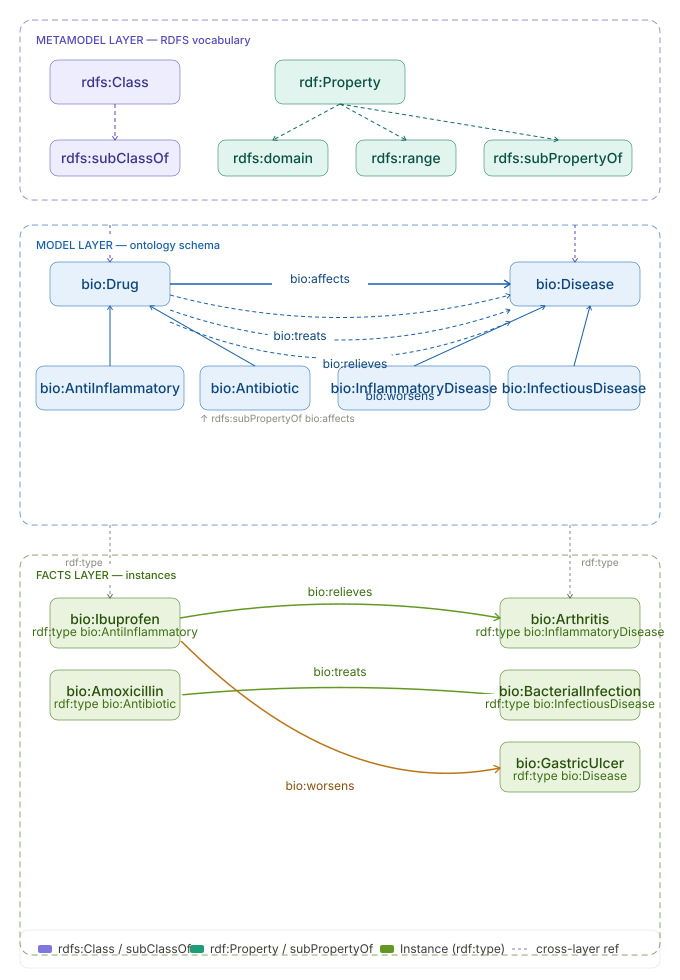
\includegraphics[width=0.85\textwidth]{rdfs_biomedical_kg_three_layers.svg}
  \textit{[See Diagram\_lab2.drawio — Metamodel layer tab]}
  \caption{Metamodel layer: RDF/RDFS constructs structuring the graph.}
  \label{fig:metamodel}
\end{figure}

% ── A.3 ──────────────────────────────────────────────────────────────────────
\subsection{Model Layer}

The model layer defines the \emph{domain-specific} taxonomy: which classes
exist and how they are related, and which properties constitute the vocabulary.

\subsubsection*{Class Hierarchy}

\begin{verbatim}
bio:Drug
    bio:AntiInflammatory
    bio:Antibiotic
    bio:Analgesic
    bio:Antiviral
    bio:Steroid

bio:Disease
    bio:InflammatoryDisease
    bio:InfectiousDisease
    bio:ChronicDisease
    bio:NeurologicalDisease
\end{verbatim}

Each subclass is declared with \texttt{rdfs:subClassOf} pointing to its
immediate parent.  No deeper nesting is introduced here because the assignment
scope does not require it; the four drug groups and four disease groups
provide sufficient semantic granularity to demonstrate RDFS reasoning.

\subsubsection*{Property Hierarchy}

\begin{verbatim}
bio:affects          (domain: bio:Drug  |  range: bio:Disease)
    bio:treats       -- subPropertyOf bio:affects
    bio:relieves     -- subPropertyOf bio:affects
    bio:worsens      -- subPropertyOf bio:affects
\end{verbatim}

The three specific properties capture semantically distinct relationships.
\texttt{treats} denotes a therapeutic action aimed at curing or eliminating a
disease (typically antibiotics/antivirals curing infections).
\texttt{relieves} denotes symptom alleviation without necessarily curing the
underlying condition (e.g., NSAIDs relieving arthritis pain).
\texttt{worsens} captures contraindications — situations where a drug
negatively affects a co-morbid condition (e.g., ibuprofen worsening chronic
kidney disease).

% ── A.4 ──────────────────────────────────────────────────────────────────────
\subsection{Facts Layer}

\subsubsection*{Instances}

The graph contains exactly \textbf{100 instances}: 50 drugs spread across the
five drug subclasses, and 50 diseases spread across the four disease subclasses.
Table~\ref{tab:instances} summarizes the counts.

\begin{table}[h!]
\centering
\caption{Instance distribution across leaf classes.}
\label{tab:instances}
\begin{tabular}{@{}llr@{}}
\toprule
\textbf{Root class} & \textbf{Subclass} & \textbf{Count} \\
\midrule
\multirow{5}{*}{Drug}    & AntiInflammatory & 10 \\
                         & Antibiotic       & 10 \\
                         & Analgesic        & 10 \\
                         & Antiviral        & 10 \\
                         & Steroid          & 10 \\
\midrule
\multirow{4}{*}{Disease} & InflammatoryDisease  & 13 \\
                         & InfectiousDisease    & 13 \\
                         & ChronicDisease       & 12 \\
                         & NeurologicalDisease  & 12 \\
\midrule
\multicolumn{2}{l}{\textbf{Total}} & \textbf{100} \\
\bottomrule
\end{tabular}
\end{table}

\subsubsection*{Explicit Relationship Triples}

Each instance is typed to exactly one leaf class using \texttt{rdf:type}.
Relationship triples use only the three specific subproperties (\texttt{treats},
\texttt{relieves}, \texttt{worsens}) — the \texttt{affects} property is
\emph{never asserted explicitly} between instances.  GraphDB's RDFS reasoner
will derive all \texttt{affects} triples automatically via the
\texttt{subPropertyOf} rule.  A sample of the explicit facts is shown below:

\begin{lstlisting}[style=turtle, caption={Sample Turtle triples from the facts layer.}]
bio:Ibuprofen       rdf:type          bio:AntiInflammatory .
bio:Ibuprofen       bio:relieves      bio:Arthritis .
bio:Ibuprofen       bio:relieves      bio:Migraine .
bio:Ibuprofen       bio:worsens       bio:ChronicKidneyDisease .

bio:Amoxicillin     rdf:type          bio:Antibiotic .
bio:Amoxicillin     bio:treats        bio:Pneumonia .
bio:Amoxicillin     bio:treats        bio:Cholera .

bio:Remdesivir      rdf:type          bio:Antiviral .
bio:Remdesivir      bio:treats        bio:COVID19 .

bio:Gabapentin      rdf:type          bio:Analgesic .
bio:Gabapentin      bio:relieves      bio:Neuropathy .
bio:Gabapentin      bio:relieves      bio:Epilepsy .

bio:Arthritis       rdf:type          bio:InflammatoryDisease .
bio:COVID19         rdf:type          bio:InfectiousDisease .
\end{lstlisting}

In total the graph contains 76 explicit relationship triples (29 \texttt{treats},
33 \texttt{relieves}, 14 \texttt{worsens}) and 205 triples overall including the
metamodel and model declarations.

% ── A.5 ──────────────────────────────────────────────────────────────────────
\subsection{Design Justifications}

\paragraph{Why a property hierarchy for \texttt{affects}?}
A single abstract property \texttt{affects} unifies the three specific
relationships under one semantic umbrella.  This lets users write a single
SPARQL query for "all drug–disease interactions" without knowing in advance
whether the relationship is therapeutic, symptomatic, or contraindicated.
Without this hierarchy, a query would need a \texttt{UNION} of three triple
patterns; with it, querying \texttt{bio:affects} suffices.

\paragraph{Why minimise explicit triples?}
The quality criterion for this assignment is to rely on RDFS inference rather
than asserting every derivable triple.  We never assert
\texttt{bio:Ibuprofen rdf:type bio:Drug} explicitly — GraphDB derives it from
\texttt{Ibuprofen rdf:type AntiInflammatory} and
\texttt{AntiInflammatory rdfs:subClassOf Drug}.
Similarly, we never assert \texttt{bio:Ibuprofen bio:affects bio:Arthritis}
— GraphDB derives it from
\texttt{Ibuprofen relieves Arthritis} and
\texttt{relieves subPropertyOf affects}.
This approach reduces graph size, eliminates the risk of inconsistent
redundancies, and tests whether the reasoning engine operates correctly.

\paragraph{Why \texttt{rdfs:domain} and \texttt{rdfs:range} only on \texttt{affects}?}
Declaring constraints at the most general level and relying on inheritance
prevents repeating them on each subproperty.  RDFS does not mandate that
subproperties inherit domain/range, but GraphDB's RDFS (Optimized) ruleset
does apply the standard RDFS-entailment rules (rdfs4, rdfs7, rdfs9) so this
works as expected.

\paragraph{Why five drug subclasses and four disease subclasses?}
The number of subclasses was chosen to reflect clinically meaningful groupings
(anti-inflammatories, antibiotics, analgesics, antivirals, steroids) while
keeping the graph tractable.  Steroids are separated from
anti-inflammatories because their mechanism of action (corticosteroid pathway)
differs from NSAIDs, which are the canonical anti-inflammatory agents.

% ── A.6 ──────────────────────────────────────────────────────────────────────
\subsection{RDFS Knowledge Graph vs.\ Neo4j Property Graph}

Table~\ref{tab:comparison} compares the two paradigms on the axes most relevant
to this assignment.

\begin{table}[h!]
\centering
\caption{RDFS knowledge graph vs.\ Neo4j property graph.}
\label{tab:comparison}
\renewcommand{\arraystretch}{1.3}
\begin{tabular}{@{}p{3.2cm}p{5.4cm}p{5.4cm}@{}}
\toprule
\textbf{Aspect} & \textbf{RDFS Knowledge Graph} & \textbf{Neo4j Property Graph} \\
\midrule
\textbf{Class hierarchy} &
  Explicit \texttt{rdfs:subClassOf} chain; querying a parent class returns all
  subclass instances automatically. &
  Node labels are flat; no inheritance.  A query for \texttt{Drug} returns only
  nodes with that exact label — not \texttt{Antibiotic} nodes unless explicitly
  listed. \\
\textbf{Property hierarchy} &
  \texttt{rdfs:subPropertyOf} means a query on \texttt{affects} returns
  \texttt{treats}, \texttt{relieves}, and \texttt{worsens} results. &
  Relationship types are independent; a \texttt{MATCH (d)-[:affects]->()} query
  finds nothing unless that type was created explicitly.  A \texttt{UNION} of
  the three specific types is required. \\
\textbf{Inference} &
  RDFS entailment rules run automatically at query time (or during materialisation).
  No extra query complexity. &
  No built-in inference engine.  Every derivable fact must be either asserted
  explicitly or reconstructed at query time via extra \texttt{MATCH} clauses. \\
\textbf{Schema standards} &
  W3C RDF/RDFS; machine-interpretable, interoperable, integrable with OWL. &
  Proprietary Labeled Property Graph model; optimised for graph traversal but
  not for semantic interoperability. \\
\textbf{Minimising redundancy} &
  Facts are stated once at the most specific level; all generalizations are
  inferred. &
  Every fact that should be queryable must be explicitly present.  A new drug
  class requires updating all queries that should match it. \\
\bottomrule
\end{tabular}
\end{table}

\noindent \textbf{Key gap}: the capability that RDFS provides and Neo4j does not is
\emph{ontological inference} — the ability to derive new facts from structural
constraints (subclass, subproperty, domain, range) without rewriting queries
or duplicating data.  A Neo4j property graph can store the same raw facts, but
it cannot answer ``find all drugs that affect any disease'' without a
programmer explicitly enumerating every relationship type in the query.

% ─────────────────────────────────────────────────────────────────────────────
\section{Section B — Implementation}
% ─────────────────────────────────────────────────────────────────────────────

\subsection{Python Script}

The knowledge graph is built programmatically with the \texttt{rdflib} Python
library (file: \texttt{build\_kg.py}) and serialised to
\texttt{biomedical\_kg.ttl} in Turtle format.

The script is organised in four logical blocks:

\begin{enumerate}[noitemsep]
  \item \textbf{Metamodel declarations} — \texttt{rdfs:Class},
        \texttt{rdfs:subClassOf}, \texttt{rdf:Property},
        \texttt{rdfs:subPropertyOf}, \texttt{rdfs:domain}, \texttt{rdfs:range}.
  \item \textbf{Instance typing} — one \texttt{rdf:type} triple per instance
        pointing to the most specific (leaf) class.
  \item \textbf{Relationship triples} — \texttt{treats}, \texttt{relieves},
        \texttt{worsens} facts derived from clinical knowledge.
  \item \textbf{Serialisation} — \texttt{g.serialize(format="turtle")} writes
        the Turtle file.
\end{enumerate}

A representative excerpt:

\begin{lstlisting}[style=python, caption={Core structure of build\_kg.py.}]
from rdflib import Graph, Namespace, RDF, RDFS

BIO = Namespace("http://www.example.org/biomedical#")
g = Graph()
g.bind("bio", BIO)

# Metamodel
g.add((BIO.Drug,    RDF.type, RDFS.Class))
g.add((BIO.Disease, RDF.type, RDFS.Class))
g.add((BIO.AntiInflammatory, RDFS.subClassOf, BIO.Drug))

g.add((BIO.affects,  RDF.type,           RDF.Property))
g.add((BIO.affects,  RDFS.domain,        BIO.Drug))
g.add((BIO.affects,  RDFS.range,         BIO.Disease))
g.add((BIO.treats,   RDFS.subPropertyOf, BIO.affects))
g.add((BIO.relieves, RDFS.subPropertyOf, BIO.affects))
g.add((BIO.worsens,  RDFS.subPropertyOf, BIO.affects))

# Facts (sample)
g.add((BIO.Ibuprofen,    RDF.type,       BIO.AntiInflammatory))
g.add((BIO.Ibuprofen,    BIO.relieves,   BIO.Arthritis))
g.add((BIO.Amoxicillin,  BIO.treats,     BIO.Pneumonia))
g.add((BIO.Ibuprofen,    BIO.worsens,    BIO.ChronicKidneyDisease))

g.serialize(destination="biomedical_kg.ttl", format="turtle")
\end{lstlisting}

\subsection{Graph Statistics}

\begin{table}[h!]
\centering
\caption{Triple counts in the generated graph.}
\begin{tabular}{@{}lr@{}}
\toprule
\textbf{Category} & \textbf{Count} \\
\midrule
Drug instances (\texttt{rdf:type} leaf class)    & 50 \\
Disease instances (\texttt{rdf:type} leaf class) & 50 \\
\texttt{treats} relationships                    & 29 \\
\texttt{relieves} relationships                  & 33 \\
\texttt{worsens} relationships                   & 14 \\
Metamodel and model declarations                 & 29 \\
\midrule
\textbf{Total triples in .ttl file}              & \textbf{205} \\
\bottomrule
\end{tabular}
\end{table}

\subsection{GraphDB Repository Setup}

\begin{enumerate}[noitemsep]
  \item Open GraphDB Workbench at \texttt{http://localhost:7200/}.
  \item Create a new repository: choose \textbf{GraphDB Repository}, set
        ID to \texttt{biomedical}, select ruleset
        \textbf{RDFS (Optimized)}.
  \item Under \emph{Advanced}, set JVM options:
        \texttt{-Xmx2000m} and
        \texttt{graphdb.workbench.maxUploadSize=40000000000}.
  \item Import \texttt{biomedical\_kg.ttl} via \emph{Import → RDF Files}.
  \item Verify inferred triples are present by running the SPARQL queries
        in Section C.
\end{enumerate}

% ─────────────────────────────────────────────────────────────────────────────
\section{Section C — Querying}
% ─────────────────────────────────────────────────────────────────────────────

\subsection{Query 1 — List All Drugs}

\begin{lstlisting}[style=sparql, caption={SPARQL: list all drugs.}]
PREFIX bio: <http://www.example.org/biomedical#>
PREFIX rdf: <http://www.w3.org/1999/02/22-rdf-syntax-ns#>

SELECT DISTINCT ?drug
WHERE {
    ?drug rdf:type bio:Drug .
}
ORDER BY ?drug
\end{lstlisting}

\begin{lstlisting}[style=cypher, caption={Cypher equivalent: list all drugs.}]
MATCH (d:Drug)
RETURN d.name AS drug
ORDER BY drug
\end{lstlisting}

\textbf{Expected result}: 50 drugs.

\textbf{Inferences applied by GraphDB}:
This query relies on the RDFS rule \textbf{rdfs9} (subclass propagation):
if \texttt{X rdfs:subClassOf Y} and \texttt{a rdf:type X}, then infer
\texttt{a rdf:type Y}.
None of the 50 drug instances are explicitly typed as \texttt{bio:Drug}; they
are typed as \texttt{AntiInflammatory}, \texttt{Antibiotic}, etc.  GraphDB
materialises \texttt{?drug rdf:type bio:Drug} for all 50 instances through the
chain \texttt{AntiInflammatory rdfs:subClassOf Drug}, etc.

\textbf{Neo4j comparison}: In Neo4j each node must carry the \texttt{Drug} label
explicitly (or a query must \texttt{UNION} all subtype labels).  There is no
equivalent inheritance mechanism; the developer must maintain redundant labels
or write more complex queries.

\subsection{Query 2 — List All Diseases}

\begin{lstlisting}[style=sparql, caption={SPARQL: list all diseases.}]
PREFIX bio: <http://www.example.org/biomedical#>
PREFIX rdf: <http://www.w3.org/1999/02/22-rdf-syntax-ns#>

SELECT DISTINCT ?disease
WHERE {
    ?disease rdf:type bio:Disease .
}
ORDER BY ?disease
\end{lstlisting}

\begin{lstlisting}[style=cypher, caption={Cypher equivalent: list all diseases.}]
MATCH (d:Disease)
RETURN d.name AS disease
ORDER BY disease
\end{lstlisting}

\textbf{Expected result}: 50 diseases.

\textbf{Inferences applied by GraphDB}: Identical mechanism to Query 1 —
RDFS rule rdfs9 propagates \texttt{rdf:type bio:Disease} to all instances
typed as \texttt{InflammatoryDisease}, \texttt{InfectiousDisease},
\texttt{ChronicDisease}, and \texttt{NeurologicalDisease}.

\subsection{Query 3 — All (Drug, Disease) Pairs Where Drug Affects Disease}

\begin{lstlisting}[style=sparql, caption={SPARQL: all drug--disease interaction pairs.}]
PREFIX bio: <http://www.example.org/biomedical#>

SELECT DISTINCT ?drug ?disease
WHERE {
    ?drug bio:affects ?disease .
}
ORDER BY ?drug ?disease
\end{lstlisting}

\begin{lstlisting}[style=cypher, caption={Cypher equivalent: all drug--disease interactions.}]
MATCH (d)-[r:TREATS|RELIEVES|WORSENS]->(dis)
RETURN d.name AS drug, dis.name AS disease
ORDER BY drug, disease
\end{lstlisting}

\textbf{Expected result}: 76 pairs (29 treats + 33 relieves + 14 worsens).

\textbf{Inferences applied by GraphDB}:
This query relies on the RDFS rule \textbf{rdfs7} (subproperty propagation):
if \texttt{P rdfs:subPropertyOf Q} and \texttt{a P b}, then infer
\texttt{a Q b}.
No \texttt{bio:affects} triple is ever explicitly asserted; all 76 are
inferred.  For example:
\begin{itemize}[noitemsep]
  \item \texttt{bio:Ibuprofen bio:relieves bio:Arthritis} (explicit)
        $\Rightarrow$ \texttt{bio:Ibuprofen bio:affects bio:Arthritis} (inferred).
  \item \texttt{bio:Amoxicillin bio:treats bio:Pneumonia} (explicit)
        $\Rightarrow$ \texttt{bio:Amoxicillin bio:affects bio:Pneumonia} (inferred).
\end{itemize}

Additionally, \texttt{rdfs:domain} and \texttt{rdfs:range} on
\texttt{bio:affects} enable GraphDB to infer (via rdfs2/rdfs3) that any
subject of an \texttt{affects} triple is a \texttt{Drug} and any object is a
\texttt{Disease}, which further enriches the graph with additional
\texttt{rdf:type} assertions.

\textbf{Neo4j comparison}: The Cypher query must enumerate every specific
relationship type explicitly.  If a new type (e.g., \texttt{PREVENTS}) is
added later, every query that should match it must be updated.  The RDFS graph
only requires declaring the new property as \texttt{rdfs:subPropertyOf affects};
all existing queries remain correct automatically.

\subsection{Summary of Inferred Triple Patterns}

\begin{table}[h!]
\centering
\caption{Inferred triple patterns and the RDFS rules that produce them.}
\renewcommand{\arraystretch}{1.3}
\begin{tabular}{@{}p{5cm}p{3.2cm}p{5cm}@{}}
\toprule
\textbf{Pattern} & \textbf{Rule} & \textbf{Example} \\
\midrule
\texttt{?x rdf:type bio:Drug} inferred from subclass &
rdfs9 &
\texttt{Ibuprofen rdf:type Drug} from \texttt{AntiInflammatory subClassOf Drug} \\
\texttt{?x rdf:type bio:Disease} inferred from subclass &
rdfs9 &
\texttt{Arthritis rdf:type Disease} from \texttt{InflammatoryDisease subClassOf Disease} \\
\texttt{?d bio:affects ?dis} inferred from subproperty &
rdfs7 &
\texttt{Ibuprofen affects Arthritis} from \texttt{relieves subPropertyOf affects} \\
\texttt{?d rdf:type bio:Drug} from domain &
rdfs2 &
Any subject of a \texttt{treats/relieves/worsens} triple inferred to be a Drug \\
\texttt{?d rdf:type bio:Disease} from range &
rdfs3 &
Any object of a \texttt{treats/relieves/worsens} triple inferred to be a Disease \\
\bottomrule
\end{tabular}
\end{table}

All of the above patterns match expectations: the RDFS (Optimized) ruleset in
GraphDB implements the full RDFS entailment regime, so every derivable triple
is materialised before queries run.

\end{document}
